\section{Hypothesentests}
Basierend auf n unabhängig und identisch Verteilte (i.i.d) Zufallsvariablen $ X_{1}, ..., X_{n} $(Messungen) soll eine Entscheidung getroffen werden, ob eine Hypothese für einen unbekannten Erwartungswert $ \mu $ gültig ist or nicht.
\subsection{Def}
$\alpha $ = Signifikanzniveau/ Fehlerwahrscheinlichkeit 
TG = Prüfgröße; 
TG* = standardisierte Prüfgröße; 
siginifikante Schlussfolgerung = $ H_{0} $ verworfen $\rightarrow$ klassischer Parametertest; 
schwache Schlussfolgerung = $ H_{0} $ wird nicht verworfen $\rightarrow$ klassischer Parametertest.
\subsection{Null- und Gegenhypothese}
\textbf{Modell:} Verteilung der Grundgesamtheit or Testgröße \textbf{TG} ( häufig $\overline{x}$ ) ist bekannt bis auf einen Parameter, z.B. $ \mu $, für den eine Hypothese aufgestellt wird.
$ TG \sim  N_{\mu, \sigma^2}$; 
\textbf{Nullhypothese: $ H_{0}$:} Angezweifelte Aussage, der widersprochen werden kann, wenn die Stichprobe einen Gegenbeweis liefert. $ H_{0}: \mu = \mu_{0}$; 
\textbf{Gegenhypothese $ H_{1} $:} Gegenteil von $ H_{0} $ z.B. $ H_{1} \neq \mu_{0} $;
\subsection{Ablehnungsbereich, Fehler 1. \& 2.}
Treffen der Testentscheidung, basierend auf einer konkreten Stichprobe 
$ \{x_{1}, ..., x_{n} \} $; Berechnung der Realisation $ tg = TG(x_{1},..., _x{n}) $ der Prüfgröße TG; 
\textbf{Ablehnungsbereich / Kritischer Bereich C}: Werte der Testgröße, die für H1, sprechen \& bei Gültigkeit von $ H_{0} $ mit Wahrscheinlichkeit $ \le \alpha $ ( meist 0.1, 0.05, or 0.01) auftreten.\textbf{Fehler 1. Art:}$ \alpha $ ist die Wahrscheinlichkeit, dass $ H_{0} $ verworfen wird, obwohl sie richtig ist.
\textbf{Annahmebereich:} Komplement $ \overline{C} $ des Ablehnungsbereichs. $ H_{0} $ kann nicht abgeleht werden, falls $ tg \in \overline{C} (P(tg \in \overline{C}) \ge 1 - \alpha) $.\textbf{Fehler 2. Art:} Die Wahrscheinlichkeit, dass $ H_{0} $ nicht abgelehnt wird, obwohl sie falsch ist.
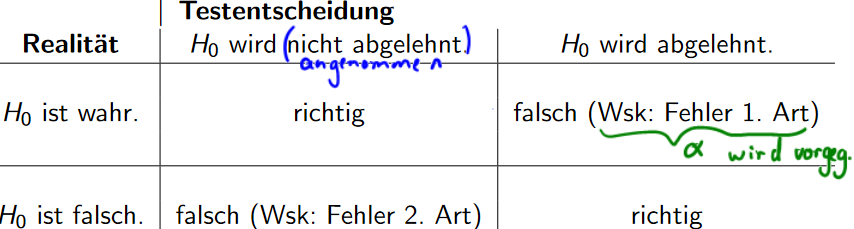
\includegraphics[scale=0.25]{./pic/Testzenarien.png}
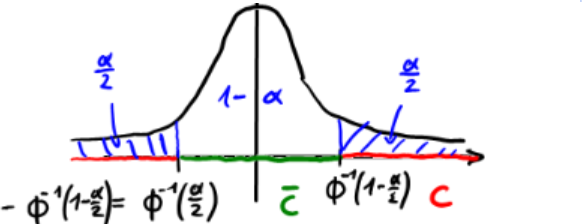
\includegraphics[scale=0.25]{./pic/StandardnormvalverteilungTestgroese.png}
$H_{0}: \mu = \mu_{0} $; $ H_{1}: \mu \neq \mu_{0} $; 
\subsection{Klassischer Parametertest}
$H_{0} $ wird abgelehnt, falls $ tg = TG( x_{1}, ..., x_{n} ) \in C $; 
$ H_{0} $ wird angenommen falls $ tg = TG(x_{1}, ..., x_{n}) \in \overline{C} $; 
Der kritische Bereich ergibt sich analog zu den Konfidenzintervallen durch die Vorgabe eines kleinen Signifikanzniveau $ \alpha $ d.h. max. Wahrscheinlichkeit für Fehler 1. Art, mit standardisierter Prüfgröße TG* gilt:
$ P (TG \in C) \le \alpha  \Leftrightarrow TG^{*} \in ]-\infty; \phi^{-1}(1- \frac{\alpha}{2}) [ \cup ] \phi^{-1}(1-\frac{\alpha}{2}); \infty [$; 
$ P(TG \in \overline{C}) \ge 1 - \alpha \Leftrightarrow TG^{*} \in [ \phi^{-1}(\frac{\alpha}{2}), \phi^{-1}(1-\frac{\alpha}{2}) ] $; 
Wird dann $ H_{0} $ verworfen, spricht man von einer signifikanten Schlussfolgerung. Kann $ H_{0} $ nicht verworfen werden, dann lässt sich keine Aussage über den Fehler 2. Art treffen \& man spricht von einer schwachen Schlussfolgerung.
\subsection{Zweiseitiger Gauß Test}
$ H_{0}: \mu = \mu_{0}  $ gegen $ H_{1}: \mu \neq \mu_{0} $; 
$ \overline{ X } \sim  N_{ \mu_{0}, \sigma_{0}^2 /n} \Rightarrow \frac{ \overline{X} - \mu_{0} }{ \sigma_{0} } \sqrt{n} \sim N_{0, 1} $; 
$ P_{ \mu0}( \overline{X} \in C ) \le \alpha \Leftrightarrow |TG| = \frac{ | \overline{X} - \mu_{0} | }{ \sigma_{0} } \sqrt{n} > \phi^{-1}(1-\frac{ \alpha}{2} )$; 
\textbf{Testentscheidung:} $ H_{0} $ wird abgelehnt, falls $ |TG| > \phi^{-1}(1-\frac{ \alpha }{ 2 } ) $; $ H_{0} $ wird angenommen, falls $ |TG| \le \phi^{-1}(1-\frac{ \alpha }{2} )$
\subsection{Einseitiger Gauß Test}
\subsubsection{linksseitig}
$ H_{0}: \mu \ge \mu_{0} $ gegen $ H_{1}: \mu  < \mu_{0}$
\subsubsection{rechtsseitig}
$ H_{0}: \mu \le \mu_{0} $ gegen $ H_{1}: \mu > \mu_{0} $
\hrule
$ P_{\mu 0} ( \overline{X} \in C ) \le \alpha \Leftrightarrow TG = \frac{ \overline{ X } - \mu_{0} }{ \sigma_{0} } \sqrt{n} < \phi^{-1} ( \alpha ) $; 
\textbf{Testentscheidung:} $ H_{0} $ wird abgelehnt falls, $ TG < \phi^{-1} ( \alpha )$; 
$ H_{0} $ wird angenommen, falls $ TG \ge \phi^{-1} ( \alpha ) $; 
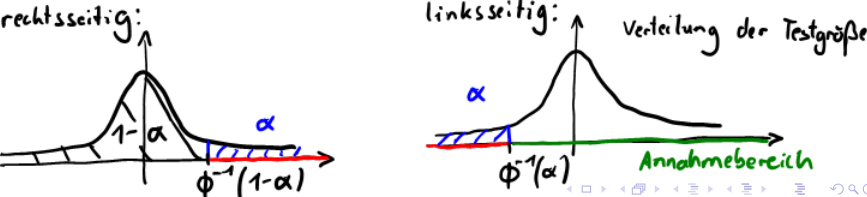
\includegraphics[scale=0.25]{./pic/EinseitigerGausTest.png}